\documentclass[12pt,a4paper]{article}
\usepackage[polish]{babel}
\usepackage[T1]{fontenc}
\usepackage[utf8x]{inputenc}
\usepackage{hyperref}
\usepackage{url}
\usepackage{graphicx}

\addtolength{\hoffset}{-1.5cm}
\addtolength{\marginparwidth}{-1.5cm}
\addtolength{\textwidth}{3cm}
\addtolength{\voffset}{-1cm}
\addtolength{\textheight}{2.5cm}
\setlength{\topmargin}{0cm}
\setlength{\headheight}{0cm}

\begin{document}
	
	\title{Systemy Sztucznej Inteligencji\\\small{dokumentacja projektu Unity Neural Network Car}}
	\author{Artur Bednarczyk, Dawid Grajewski, grupa A}
	\date{\today}

	\maketitle
	\newpage
	\section*{Część I}
	\subsection*{Opis programu}
	Tutaj, nasz super opis, jaki ten program jest cudowny i superowy. Nikt nie ma tak fajnego autka, które tak fajnie pędzi przez super fajny tor.
	Panie, inne autka tak nie pojadą jak nasze. Niżej jakiś normalny opis się zacznie;// \\
	
	Unity Nueral Network Car jest symulacją jazdy samochodu na torze. Samochód jest autonomiczny, co oznacza, że użytkownik nie musi go kontrolować, pojedzie sam. Samochód został nauczony jak jeździć dzięki specjalnie zaprojektowanej sieci neuronowej, dzięki czemu może jeździć po naszym torze nie rozbijając się na każdym zakręcie.
	\subsection*{Instrukcja obsługi}
	Magia dzieje się sama. Nie musisz tego znać.
	\subsection*{Dodatkowe informacje}
	Fajne, co nie? Tylko co mamy na myśli, mówiąc "Dodatkowe informacyje?"
	\newpage
	\section*{Część II}
	\subsection*{Opis działania} 
	Tutaj uwzględniamy część matematyczną.
	- serio? musimy?
	No dobra, dodam tutaj te fajne wzorki jak np. ten cały sigmoid, jako nasza funkcja aktywacji:
	$$ S(x) = \frac{1}{1+e^{-x}} = \frac{e^x}{e^x+1} $$
	Jakieś randomowe wzroki z randomowych tutoriali do AI (tam mają nawalone tych wzrów wiec coś tam damy.) np. takie coś, to chyba uczenie perceptronu, czyli komórce dowalama sume wszystkich wartości pomnożonych przez wagi:
	$$ \sum_{i=1}^{n}u_iw_i $$
	
	PROPAGACJA WSTECZNA \\
	https://mattmazur.com/2015/03/17/a-step-by-step-backpropagation-example/ \\
	xD\\
	\subsection*{Algorytm}
	mile widziany pseudokod z użyciem biblioteki \LaTeX
	\\
	\\
	pseudo kod czego naszego AI tutaj sie da; o ile da rade te wszystkie rzeczy w coś krótkiego zwinąć, bo inaczej jest w tym sens, skoro cały kod będzie niżej?\\
	\\
	Jak to nie będzie zbyt ogromne, to mogę zrobić ładny(jak się uda) schemat blokowy.
	\subsection*{Bazy danych}
	Należy pokazać przykładowe dane, które były wykorzystywane podczas uczenia klasyfikatorów.
	\\
	Czyli te 120 wierszy czy ile tego tam mamy? Czy wystarczy mu pokazać, że mamy dane w takiej formie i wkleić kilka wierszy tego i dać trzy kropki, o takie "...".
	\subsection*{Implementacja}
	Opis, zasada i działanie programu ze względu na podział na pliki, nastepnie	funkcje programu wraz ze szczegółowym opisem działania
	\begin{verbatim}
	proszę zwrócić uwagę na wychodzenie poza obszar kartki.
	
	No spoko, ja tu dopiljnuje, żeby wyglądało po ludzku.
	\end{verbatim}
	\subsection*{Testy}
	Tutaj powinna pojawić się analiza uzyskanych wyników oraz wykresy/pomiary.
	
	No lekko, tutaj wleci super wykres nakodzony w pytonie. \\
	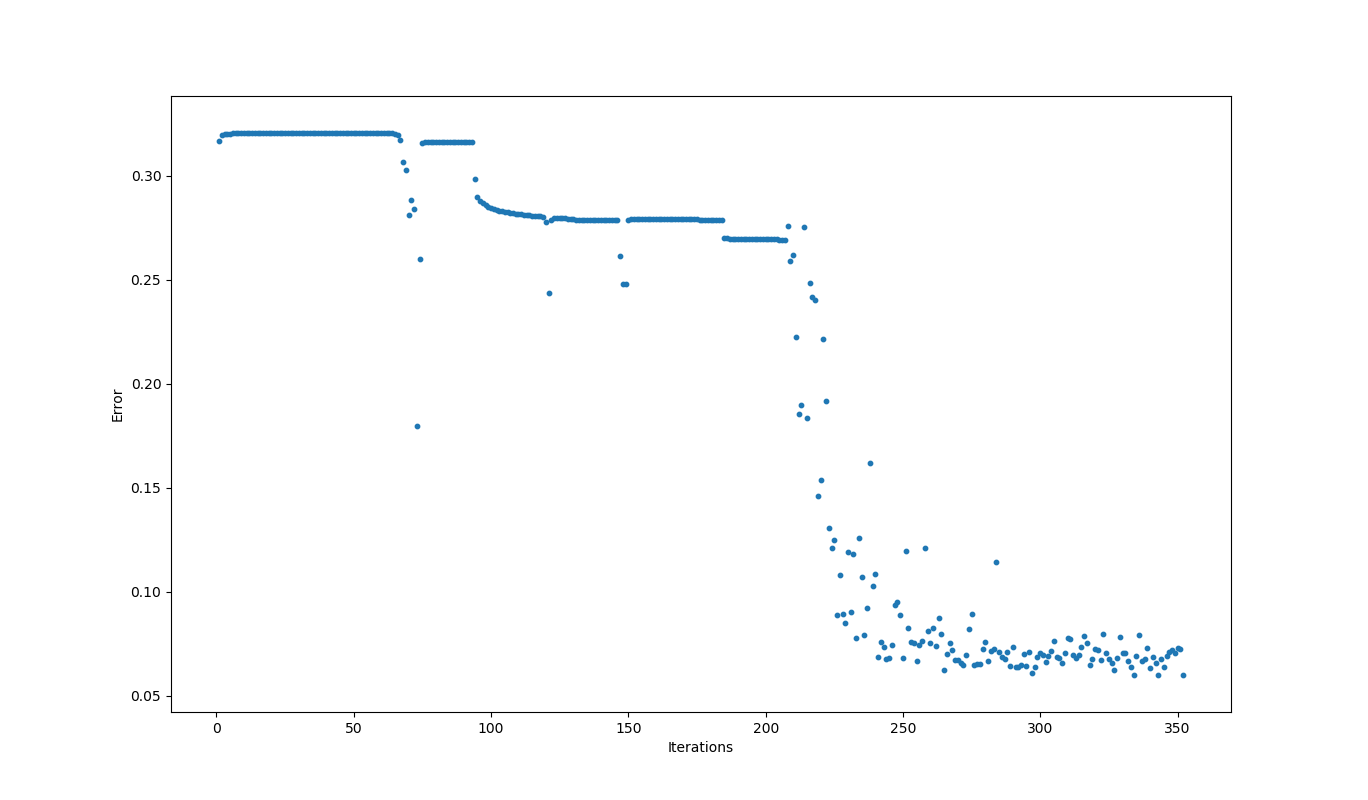
\includegraphics[scale=0.5]{supa_wykres}
	\newpage
	\section*{Pełen kod aplikacji}
	tutaj wklejamy pełen kod.\\ Dalej nie rozumiem sensu tego punktu. ale niech będzie. Pewnie wszystko będzie ważyło trochę zbyt dużo, żeby to wrzucić na platformę xD
\end{document}
